\documentclass[tikz,border=8pt]{standalone}
% Shared look for every TikZ diagram. Load with \input{../../tools/tikz-style.tex}
\usepackage[T1]{fontenc}
\usepackage{lmodern}
\renewcommand{\sfdefault}{lmr}  % diagrams use the same serif as the text
\usetikzlibrary{arrows.meta, positioning, shapes.geometric, calc, fit, backgrounds}
\definecolor{cblue}{HTML}{4C78A8}
\definecolor{corange}{HTML}{F58518}
\definecolor{cgreen}{HTML}{54A24B}
\definecolor{cred}{HTML}{E45756}
\definecolor{cpurple}{HTML}{B279A2}
\definecolor{cgrey}{HTML}{6B6B6B}
\tikzset{
  every picture/.style={font=\sffamily, line width=1.2pt},
  box/.style={draw=#1, fill=#1!12, rounded corners=4pt, align=center, inner sep=7pt, minimum height=1.1cm},
  box/.default=cgrey,
  arrow/.style={-{Stealth[length=3mm]}, draw=cgrey, line width=1.4pt},
  title/.style={font=\sffamily\bfseries\Large},
  note/.style={font=\sffamily\small, text=cgrey, align=center},
}
\AtBeginDocument{\hyphenpenalty=10000 \exhyphenpenalty=10000}

% Left: an optical wheel encoder, a disc with evenly spaced slots on the wheel shaft and a light sensor that counts a
% pulse at every slot. Right: the three steps of wheel odometry for one step of 0.1 s with the Note's numbers.
\begin{document}
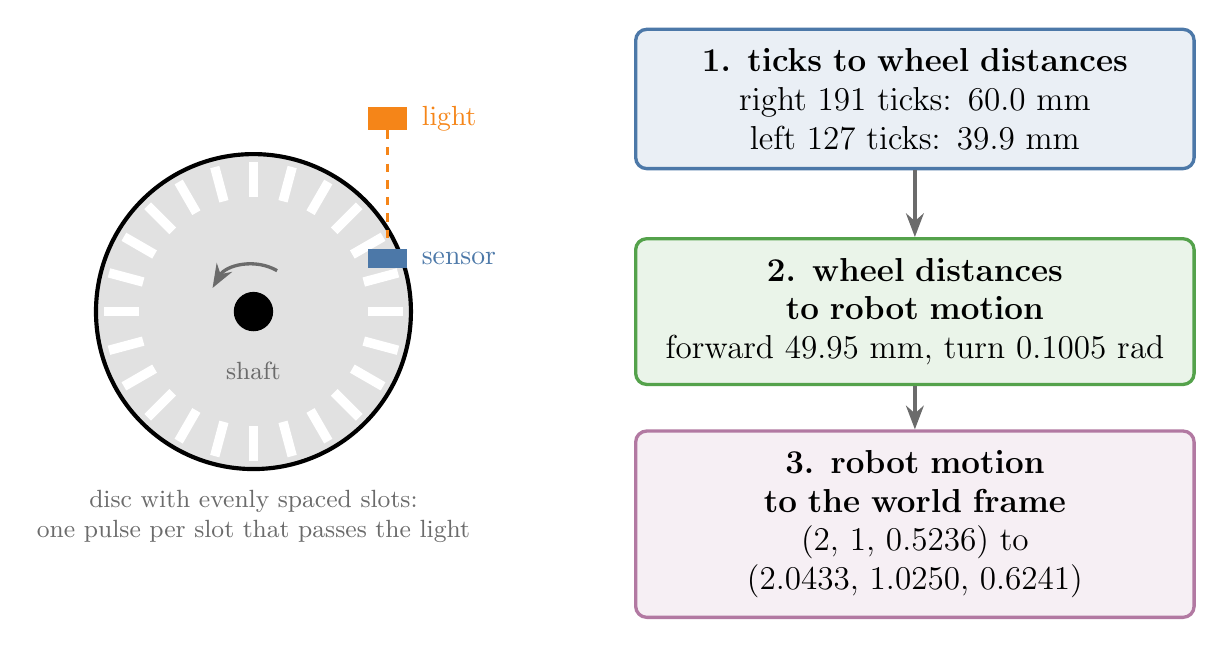
\begin{tikzpicture}[every node/.append style={font=\large}]
  % encoder disc
  \fill[cgrey!20] (0,0) circle (2);
  \draw[black, line width=1.5pt] (0,0) circle (2);
  \foreach \a in {0,15,...,345} \fill[white, rotate=\a] (1.45,-0.06) rectangle (1.9,0.06);
  \fill[black] (0,0) circle (0.25);
  \draw[cgrey, -{Stealth[length=3mm]}] (60:0.6) arc (60:150:0.6);
  \node[note] at (0,-0.75) {shaft};
  % light source and sensor
  \fill[corange] (1.45,2.3) rectangle (1.95,2.6); \node[corange, right, font=\normalsize] at (2.0,2.45) {light};
  \draw[corange, dashed, line width=1pt] (1.7,2.3) -- (1.7,0.9);
  \fill[cblue] (1.45,0.55) rectangle (1.95,0.8); \node[cblue, right, font=\normalsize] at (2.0,0.67) {sensor};
  \node[note, align=center] at (0,-2.6) {disc with evenly spaced slots:\\one pulse per slot that passes the light};
  % pipeline
  \begin{scope}[xshift=8.4cm]
    \node[box=cblue, text width=6.6cm] (a) at (0,2.7) {\textbf{1. ticks to wheel distances}\\right 191 ticks: 60.0 mm\\left 127 ticks: 39.9 mm};
    \node[box=cgreen, text width=6.6cm] (b) at (0,0) {\textbf{2. wheel distances to robot motion}\\forward 49.95 mm, turn 0.1005 rad};
    \node[box=cpurple, text width=6.6cm] (c) at (0,-2.7) {\textbf{3. robot motion to the world frame}\\(2, 1, 0.5236) to (2.0433, 1.0250, 0.6241)};
    \draw[arrow] (a) -- (b); \draw[arrow] (b) -- (c);
  \end{scope}
\end{tikzpicture}
\end{document}
